% Options for packages loaded elsewhere
\PassOptionsToPackage{unicode}{hyperref}
\PassOptionsToPackage{hyphens}{url}
%
\documentclass[
]{article}
\usepackage{amsmath,amssymb}
\usepackage{lmodern}
\usepackage{iftex}
\ifPDFTeX
  \usepackage[T1]{fontenc}
  \usepackage[utf8]{inputenc}
  \usepackage{textcomp} % provide euro and other symbols
\else % if luatex or xetex
  \usepackage{unicode-math}
  \defaultfontfeatures{Scale=MatchLowercase}
  \defaultfontfeatures[\rmfamily]{Ligatures=TeX,Scale=1}
\fi
% Use upquote if available, for straight quotes in verbatim environments
\IfFileExists{upquote.sty}{\usepackage{upquote}}{}
\IfFileExists{microtype.sty}{% use microtype if available
  \usepackage[]{microtype}
  \UseMicrotypeSet[protrusion]{basicmath} % disable protrusion for tt fonts
}{}
\makeatletter
\@ifundefined{KOMAClassName}{% if non-KOMA class
  \IfFileExists{parskip.sty}{%
    \usepackage{parskip}
  }{% else
    \setlength{\parindent}{0pt}
    \setlength{\parskip}{6pt plus 2pt minus 1pt}}
}{% if KOMA class
  \KOMAoptions{parskip=half}}
\makeatother
\usepackage{xcolor}
\usepackage[margin=1in]{geometry}
\usepackage{longtable,booktabs,array}
\usepackage{calc} % for calculating minipage widths
% Correct order of tables after \paragraph or \subparagraph
\usepackage{etoolbox}
\makeatletter
\patchcmd\longtable{\par}{\if@noskipsec\mbox{}\fi\par}{}{}
\makeatother
% Allow footnotes in longtable head/foot
\IfFileExists{footnotehyper.sty}{\usepackage{footnotehyper}}{\usepackage{footnote}}
\makesavenoteenv{longtable}
\usepackage{graphicx}
\makeatletter
\def\maxwidth{\ifdim\Gin@nat@width>\linewidth\linewidth\else\Gin@nat@width\fi}
\def\maxheight{\ifdim\Gin@nat@height>\textheight\textheight\else\Gin@nat@height\fi}
\makeatother
% Scale images if necessary, so that they will not overflow the page
% margins by default, and it is still possible to overwrite the defaults
% using explicit options in \includegraphics[width, height, ...]{}
\setkeys{Gin}{width=\maxwidth,height=\maxheight,keepaspectratio}
% Set default figure placement to htbp
\makeatletter
\def\fps@figure{htbp}
\makeatother
\setlength{\emergencystretch}{3em} % prevent overfull lines
\providecommand{\tightlist}{%
  \setlength{\itemsep}{0pt}\setlength{\parskip}{0pt}}
\setcounter{secnumdepth}{-\maxdimen} % remove section numbering
\usepackage{booktabs}
\usepackage{longtable}
\usepackage{array}
\usepackage{multirow}
\usepackage{wrapfig}
\usepackage{float}
\usepackage{colortbl}
\usepackage{pdflscape}
\usepackage{tabu}
\usepackage{threeparttable}
\usepackage{threeparttablex}
\usepackage[normalem]{ulem}
\usepackage{makecell}
\usepackage{xcolor}
\ifLuaTeX
  \usepackage{selnolig}  % disable illegal ligatures
\fi
\IfFileExists{bookmark.sty}{\usepackage{bookmark}}{\usepackage{hyperref}}
\IfFileExists{xurl.sty}{\usepackage{xurl}}{} % add URL line breaks if available
\urlstyle{same} % disable monospaced font for URLs
\hypersetup{
  pdftitle={Untitled},
  pdfauthor={Vimaljeet Singh},
  hidelinks,
  pdfcreator={LaTeX via pandoc}}

\title{Untitled}
\author{Vimaljeet Singh}
\date{2023-03-24}

\begin{document}
\maketitle

\hypertarget{introduction}{%
\subsection{Introduction}\label{introduction}}

The dataset we have chosen to analyze is Hadi Fanaee-T's
\href{https://archive.ics.uci.edu/ml/datasets/Bike+Sharing+Dataset}{Bike
Sharing Dataset}, from the Laboratory of Artificial Intelligence and
Decision Support (LIAAD), University of Porto, accessed in the UCI
Machine Learning Repository. This dataset combines the Trip History Data
for the years of 2011 and 2012 of `Capital Bikeshare', which is metro
Washington DC's bikeshare service, with weather data and the holiday
schedule. We are hypothesizing that we are able to predict the count of
bikes rented in a given hour given the predictor variables (weather,
calendar date and time, etc). We are also hypothesizing that results
will be better if we model casual user bike rentals separately than
registered users. Finally, we want to investigate which predictor
variables are most important in making the predictions.

\hypertarget{description-of-dataset}{%
\subsection{Description of Dataset}\label{description-of-dataset}}

The data consists of an aggregated count of `rides' by hour, over the
span of the years 2011 and 2012. It contains 17379 rows and 17 columns.

\begin{longtable}[]{@{}llll@{}}
\toprule()
Variable Name & Description & Type & \\
\midrule()
\endhead
instant & Record index & ordinal & \\
dteday & Date & datetime & \\
season & Season (winter, spring, summer, fall) & categorical & \\
yr & Year (2011, 2012) & ordinal & \\
mth & Month & categorical & \\
hr & Hour & categorical & \\
holiday & Whether day is a holiday or not & boolean & \\
weekday & Day of the week & categorical & \\
workingday & If day is neither weekend nor holiday & boolean & \\
weathersit & Weather conditions & ordinal & \\
temp & Temperature in Celsius & numerical & \\
atemp & Feeling temperature in Celsius & numerical & \\
hum & Humidity & numerical & \\
windspeed & Wind speed & numerical & \\
casual & Count of bikes rented by casual users & numerical & \\
registered & Count of bikes rented registered users & numerical & \\
cnt & Count of total bikes rented & numerical & \\
\bottomrule()
\end{longtable}

\hypertarget{plan-overview}{%
\subsection{Plan overview}\label{plan-overview}}

We will be conducting a linear regression, as it is the most simple
model, as well as investigating a Poisson Regression, since this is
count data, and a random forest model, to see if it improves the
predictions. We'll investigate these models for the total count, as then
separately for the casual counts and registered counts. We will
investigate outliers in the data, and we will use variable selection
methods to investigate which variables are most important. We are
separating our data into an 60/40 training/testing set, and we will be
using MSE as a measure of fit, as well as R\^{}2. Finally, we will make
our conclusions, and talk about limitations and possible future work.

In this report, we will explore different models for predicting the
rental bike count like - Linear Regression, Poisson Regression, and
Random Forests (RF). We chose these models due to their ability to
handle the type of response variable we have and their relative
simplicity, which allows for easy interpretation (except RF). We will
first fit these models on the total rental count (cnt), and then
separately on the `casual' and `registered' rental counts. To ensure
accurate predictions, we will investigate outliers in the data and use
variable selection methods to determine which predictors are most
important. Our dataset will be split into a 60/40 training/testing set,
and we will use mean squared error (MSE) and \(R^2\) as measures of fit.

Finally, we will present our conclusions and discuss the limitations of
our models, as well as possible directions for future research.

Due to high collinearity, we've decided to remove the \texttt{atemp} as
well as the \texttt{workingday} variable from our models (check the
figure below). We are considering our full model to include the
following predictors: yr, mth, hr, holiday, weekday, weathersit,
rawtemp, rawhum, and rawwindspeed, season. The response variables are
cnt, casual, and registered.

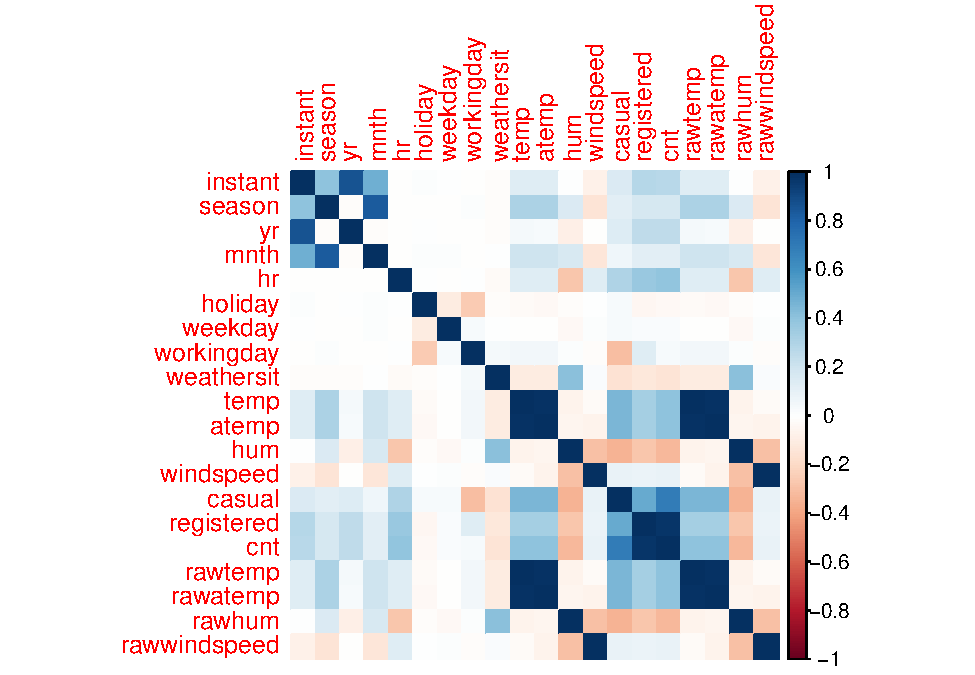
\includegraphics{test_files/figure-latex/unnamed-chunk-2-1.pdf}

\hypertarget{linear-model}{%
\subsection{Linear Model}\label{linear-model}}

In the Bike Sharing dataset, the response variable `cnt' represents the
number of hourly users of a bike. Unlike qualitative or quantitative
variables, this response takes on non-negative integer values or counts.

\begin{table}
\centering
\begin{tabular}{c|c}
\hline
Statistic & Value\\
\hline
R\_Squared & 0.6875\\
\hline
MSE & 9951.4900\\
\hline
F-Stat & 447.5300\\
\hline
\end{tabular}
\end{table}

The table above shows the statistics of the fitted linear model. The
linear model has a \(R^2\) of 0.6875 which means the model is able to
explain 68.75\% variation in the count data based on the given
independent variables. The F-statistic is very high which means one or
more of the coefficients is significant. Most of the values that are in
the model are significant. Overall, this seems to be a good fit for the
model, but there seems to be an issue with the predicted values. 9.84\%
of the fitted values are negative which means that the linear model
predicts a negative number of users during 9.84\% of the hours in the
data set (check `Linear Model Fit' chart below too). The negative
expected values of bikers in certain situations raises doubts about the
reliability of predictions made from the regression model. It also casts
doubt on the accuracy of the coefficient estimates and confidence
intervals of the model. Moreover, it is plausible to assume that when
the expected number of bikers is low, the variance associated with the
number of users should also be small. For example, during a heavy
December snow at 1 AM, we anticipate that only a few people will use a
bike, and there will be less variation in the number of users during
such conditions. In contrast, between 6am and 9am in summers, more
number of riders are expected and hence the variance should be higher.
The table below shows how these statistics vary.

\begin{table}
\centering
\begin{tabular}{c|c|c|c}
\hline
Months & Time & Riders\_Mean & Riders\_Variance\\
\hline
December, January, February & 1am - 4am & 12.10479 & 284.7236\\
\hline
April, May, June & 6am - 9am & 238.01648 & 32062.5637\\
\hline
\end{tabular}
\end{table}

Heteroscedasticity refers to a violation of the assumption in the linear
model:

\(Y = \beta_{0} + \sum\limits_{j=1} ^ {p} X_{j}\beta_{j} + \epsilon\)

where the variance of the response variable (cnt) is not constant across
the range of predictor variables. The most common form of
heteroscedasticity in the response variable is that the variance of the
response variable may change as the mean of the response variable
changes. The estimate for the variance of the slope and variance will be
inaccurate. Heteroscedasticity can be detected by examining the scatter
plot of the data before performing the regression. We will plot a graph
of mean vs variance for the `cnt' values for both the years to inspect
this.

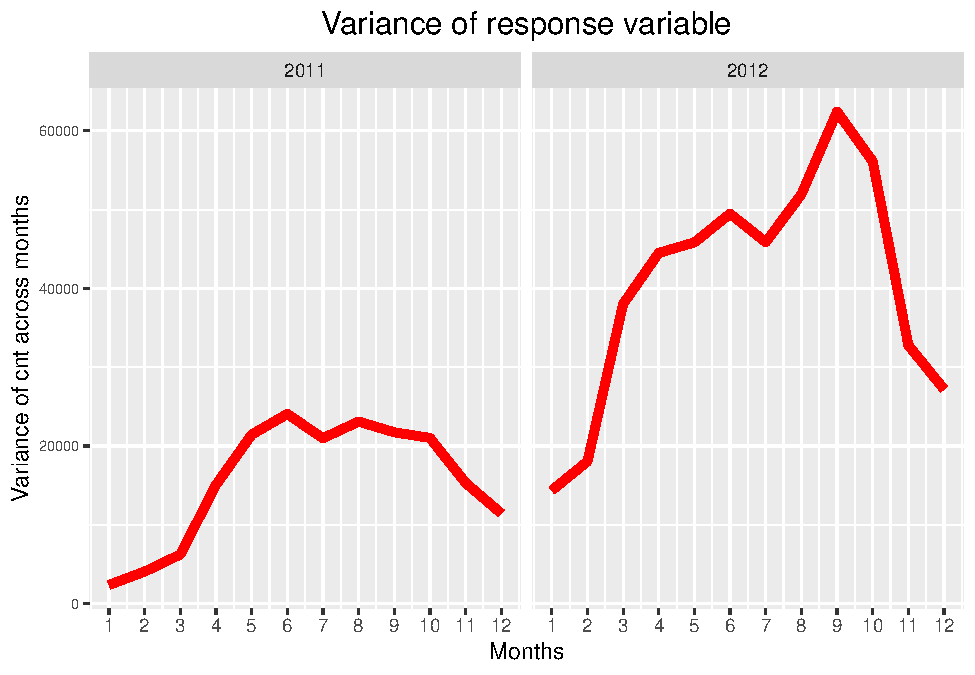
\includegraphics{test_files/figure-latex/unnamed-chunk-7-1.pdf}

The plot above clearly shows that the variance varies throughout the
year and the assumption of a linear relationship between the predictor
variable and the response variable is severely violated due to unequal
variance of the response variable. In fact, the variance in 2012 is
visibly more too on the whole. As a result, the assumption of
homoscedasticity is not met, which raises concerns about the
appropriateness of using a linear regression model to analyze the data.

The following plot shows the observed values vs predicted values using
linear model. Our concern here is visualzied when we see the red dots
falling below the 0 on the x-axis.

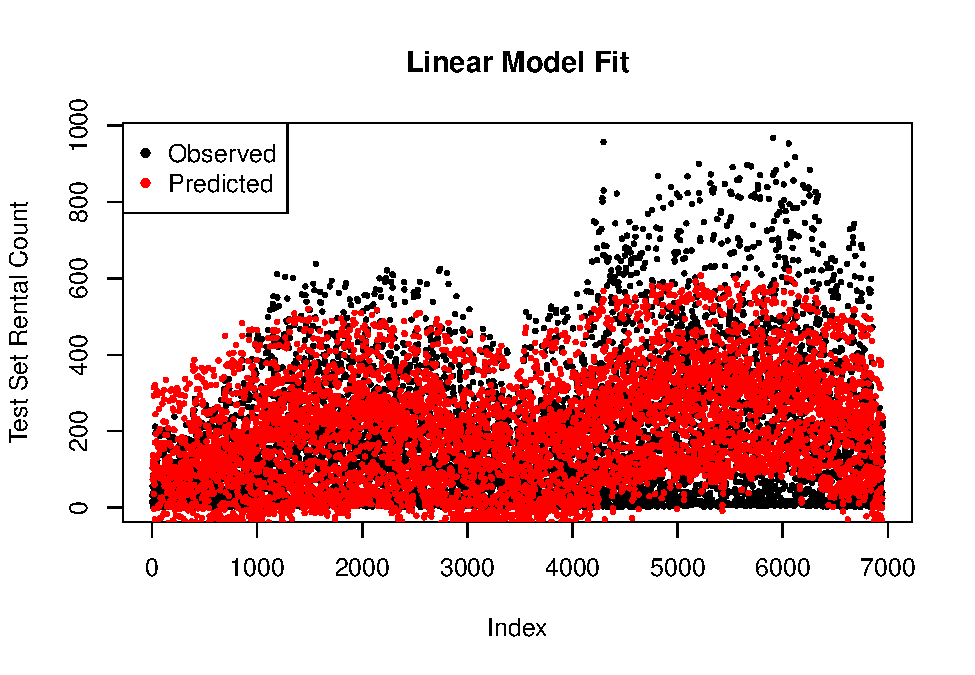
\includegraphics{test_files/figure-latex/unnamed-chunk-8-1.pdf}

We cannot have predicted count values that are negative (see the red
dots below 0 in the graph below) as the number of bikes rented in an
hour can never be negative. This is another reason we should not use
linear model for this data. Furthermore, the response in this dataset
`cnt' is in the form of integers, while a linear model assumes that the
error term is continuous. This means that the response variable in a
linear model must be continuous as well. Therefore, the integer nature
of `cnt' response implies that a linear regression model may not be
entirely suitable for this dataset.

Transforming the response into \texttt{log} could help us eradicate some
of the problems that we are facing with linear model. We could fit
something like:

\(log(cnt) = \sum\limits_{j=1} ^ {p} X_{j}\beta_{j} + \epsilon\)

Transforming the response variable in the Bikeshare data can be helpful
in addressing two main issues associated with fitting a linear
regression model: the occurrence of negative predictions and the
presence of heteroscedasticity in the original data. By transforming the
response, we can avoid negative predicted values and reduce
heteroscedasticity, resulting in a more accurate and reliable model.
While transforming the response variable can address some issues in
fitting a linear regression model, it is not entirely satisfactory. This
is because the predictions and interpretations are made in terms of the
logarithm of the response rather than the response itself, which can be
challenging for interpretation. Moreover, this transformation cannot be
applied to data sets where the response can take on a value of 0.
Therefore, although using a transformation of the response can be a
reasonable approach for some count-valued data sets, it may not always
be the optimal solution.

\hypertarget{poisson-model}{%
\subsection{Poisson Model}\label{poisson-model}}

The Poisson distribution is commonly employed to model counts due to
several reasons, such as the fact that counts, like the Poisson
distribution, are restricted to non-negative integer values. This makes
it a suitable and natural choice for modeling count data.

\begin{verbatim}
## 
## Call:
## glm(formula = cnt ~ ., family = poisson, data = df[, -c(8, 9)])
## 
## Deviance Residuals: 
##      Min        1Q    Median        3Q       Max  
## -23.5283   -3.7534   -0.8594    3.0242   22.1720  
## 
## Coefficients:
##                          Estimate Std. Error  z value Pr(>|z|)    
## (Intercept)             3.063e+00  8.505e-03  360.146  < 2e-16 ***
## seasonspring            2.589e-01  4.846e-03   53.423  < 2e-16 ***
## seasonsummer            2.401e-01  5.498e-03   43.663  < 2e-16 ***
## seasonfall              4.548e-01  5.319e-03   85.505  < 2e-16 ***
## yr1                     4.732e-01  1.492e-03  317.222  < 2e-16 ***
## mnthFeb                 1.360e-01  4.853e-03   28.033  < 2e-16 ***
## mnthMar                 2.419e-01  5.065e-03   47.761  < 2e-16 ***
## mnthApr                 2.084e-01  6.796e-03   30.665  < 2e-16 ***
## mnthMay                 2.679e-01  7.134e-03   37.559  < 2e-16 ***
## mnthJun                 2.007e-01  7.264e-03   27.623  < 2e-16 ***
## mnthJul                 1.139e-01  7.838e-03   14.533  < 2e-16 ***
## mnthAug                 2.017e-01  7.629e-03   26.437  < 2e-16 ***
## mnthSep                 3.057e-01  7.028e-03   43.502  < 2e-16 ***
## mnthOct                 1.928e-01  6.994e-03   27.563  < 2e-16 ***
## mnthNov                 6.997e-02  6.867e-03   10.189  < 2e-16 ***
## mnthDec                 6.062e-02  6.026e-03   10.059  < 2e-16 ***
## hr1                    -4.760e-01  1.058e-02  -44.992  < 2e-16 ***
## hr2                    -8.246e-01  1.205e-02  -68.423  < 2e-16 ***
## hr3                    -1.557e+00  1.567e-02  -99.340  < 2e-16 ***
## hr4                    -2.107e+00  2.059e-02 -102.343  < 2e-16 ***
## hr5                    -9.420e-01  1.248e-02  -75.486  < 2e-16 ***
## hr6                     4.097e-01  8.558e-03   47.877  < 2e-16 ***
## hr7                     1.450e+00  7.169e-03  202.227  < 2e-16 ***
## hr8                     1.919e+00  6.917e-03  277.422  < 2e-16 ***
## hr9                     1.379e+00  7.255e-03  190.052  < 2e-16 ***
## hr10                    1.132e+00  7.448e-03  152.032  < 2e-16 ***
## hr11                    1.257e+00  7.278e-03  172.685  < 2e-16 ***
## hr12                    1.468e+00  7.216e-03  203.431  < 2e-16 ***
## hr13                    1.447e+00  7.229e-03  200.104  < 2e-16 ***
## hr14                    1.382e+00  7.332e-03  188.429  < 2e-16 ***
## hr15                    1.407e+00  7.288e-03  193.095  < 2e-16 ***
## hr16                    1.623e+00  7.158e-03  226.678  < 2e-16 ***
## hr17                    2.030e+00  6.976e-03  290.988  < 2e-16 ***
## hr18                    1.980e+00  6.958e-03  284.518  < 2e-16 ***
## hr19                    1.674e+00  7.035e-03  238.015  < 2e-16 ***
## hr20                    1.383e+00  7.278e-03  190.082  < 2e-16 ***
## hr21                    1.128e+00  7.451e-03  151.403  < 2e-16 ***
## hr22                    8.672e-01  7.774e-03  111.552  < 2e-16 ***
## hr23                    4.869e-01  8.239e-03   59.094  < 2e-16 ***
## holidayHoliday         -1.808e-01  4.969e-03  -36.384  < 2e-16 ***
## weekdayMon              5.981e-02  2.804e-03   21.334  < 2e-16 ***
## weekdayTues             6.637e-02  2.701e-03   24.567  < 2e-16 ***
## weekdayWed              7.087e-02  2.700e-03   26.249  < 2e-16 ***
## weekdayThurs            6.874e-02  2.699e-03   25.473  < 2e-16 ***
## weekdayFri              9.491e-02  2.665e-03   35.607  < 2e-16 ***
## weekdaySat              8.869e-02  2.677e-03   33.127  < 2e-16 ***
## weathersitMisty        -6.095e-02  1.841e-03  -33.102  < 2e-16 ***
## weathersitLight precip -5.179e-01  3.761e-03 -137.683  < 2e-16 ***
## weathersitheavy precip -5.250e-01  7.088e-02   -7.407 1.29e-13 ***
## rawtemp                 2.205e-02  1.899e-04  116.077  < 2e-16 ***
## rawhum                 -1.586e-03  5.323e-05  -29.790  < 2e-16 ***
## rawwindspeed           -1.380e-03  9.228e-05  -14.958  < 2e-16 ***
## ---
## Signif. codes:  0 '***' 0.001 '**' 0.01 '*' 0.05 '.' 0.1 ' ' 1
## 
## (Dispersion parameter for poisson family taken to be 1)
## 
##     Null deviance: 1755788  on 10426  degrees of freedom
## Residual deviance:  343555  on 10375  degrees of freedom
## AIC: 410117
## 
## Number of Fisher Scoring iterations: 5
\end{verbatim}

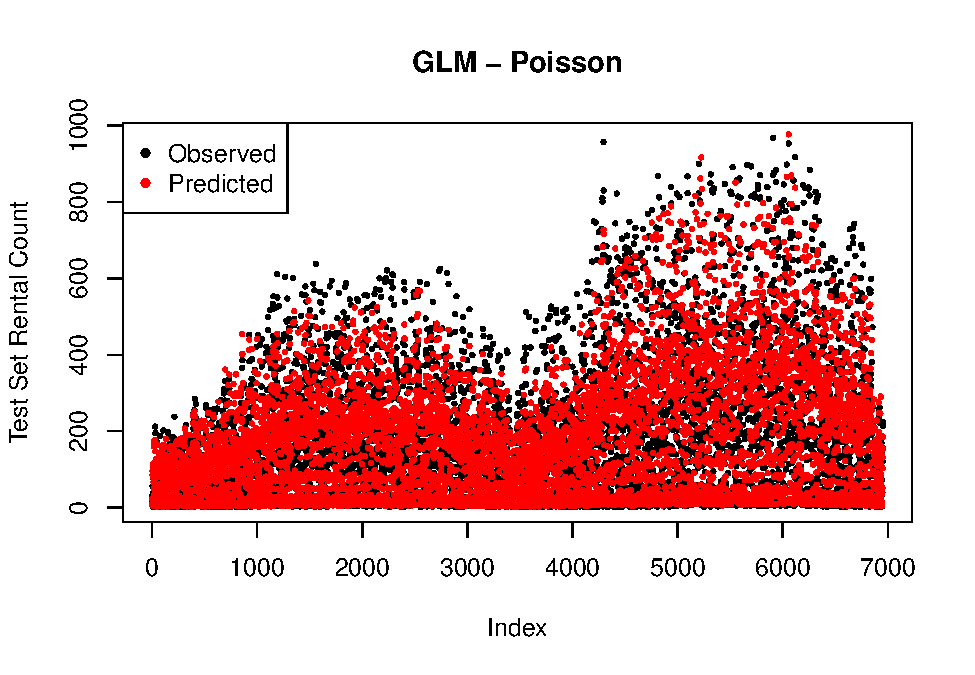
\includegraphics{test_files/figure-latex/unnamed-chunk-10-1.pdf}

When using a Poisson regression to model bike usage, we make an implicit
assumption that the mean bike usage in an hour is equal to the variance
of bike usage during that hour. This is because the Poisson distribution
is typically used to model counts, and counts, like the Poisson
distribution, take on non-negative integer values. In contrast, a linear
regression model assumes that the variance of bike usage always takes on
a constant value. Therefore, the Poisson regression model is better
suited to handle the mean-variance relationship observed in the Bike
sharing data compared to the linear regression model. In fact from the
table below, we can see that the variance in `cnt' appears to be much
higher than the mean, a situation referred to as ``overdispersion''
which can seemingly be handled by quasi-poisson model. We checked the
results from a quasi-poisson model as well and the result is exactly the
same as that of a Poisson model.

\begin{table}
\centering
\begin{tabular}{c|c|c|c}
\hline
Year & Month & Mean & Var\\
\hline
2011 & 1 & 55.51 & 2363.97\\
\hline
2011 & 2 & 74.29 & 4048.27\\
\hline
2011 & 3 & 87.73 & 6221.97\\
\hline
2011 & 4 & 131.95 & 15056.42\\
\hline
2011 & 5 & 182.56 & 21431.03\\
\hline
2011 & 6 & 199.32 & 24050.94\\
\hline
2011 & 7 & 189.97 & 20977.03\\
\hline
2011 & 8 & 186.99 & 23089.84\\
\hline
2011 & 9 & 177.71 & 21731.45\\
\hline
2011 & 10 & 166.23 & 21014.77\\
\hline
2011 & 11 & 142.10 & 15313.78\\
\hline
2011 & 12 & 117.84 & 11436.88\\
\hline
2012 & 1 & 130.56 & 14351.25\\
\hline
2012 & 2 & 149.04 & 18032.86\\
\hline
2012 & 3 & 221.90 & 38013.55\\
\hline
2012 & 4 & 242.65 & 44495.40\\
\hline
2012 & 5 & 263.26 & 45834.14\\
\hline
2012 & 6 & 281.71 & 49466.60\\
\hline
2012 & 7 & 273.67 & 45863.84\\
\hline
2012 & 8 & 288.31 & 51927.01\\
\hline
2012 & 9 & 303.57 & 62430.32\\
\hline
2012 & 10 & 280.85 & 56122.56\\
\hline
2012 & 11 & 212.62 & 32788.45\\
\hline
2012 & 12 & 166.73 & 27190.42\\
\hline
\end{tabular}
\end{table}

\end{document}
